\documentclass[10pt,letterpaper]{article}
\usepackage[utf8]{inputenc}
\usepackage{amsmath}
\DeclareMathOperator{\sign}{sgn}
\usepackage{amsfonts}
\usepackage{amssymb}
\usepackage[margin=0.5in]{geometry}
\usepackage{graphicx}
\usepackage{sidecap}
\usepackage{float}

\usepackage[font=small,labelfont=bf]{caption}


\title{\vspace{-4ex}Neural Networks\vspace{-3.5ex}}
\begin{document}
\newgeometry{top=0.75in,left=0.75in,right=0.75in,bottom=1in}
\maketitle
\vspace{-0.5em}
\begin{abstract}
In this short paper we will discuss the fundamentals of neural networks and their implementation in detail. We will give a general overview of how neural networks work, discuss calculation of the gradient and implementation of back-propagation, and test our results on some real MNIST code.
\end{abstract}
Neural networks have been around for at least a few decades, but only recently have them become popular as a method for learning parameters that can correctly translate an input into an output. This is because of increased computational power, a greater availability of training data, as well as the fact that more complex models, like deep neural nets, are actually easy to train - the same back-propagation that works to update normal neural networks works just as well for multiple hidden layers.
\begin{figure}[!htb]
\centering
\minipage{0.5\textwidth}
  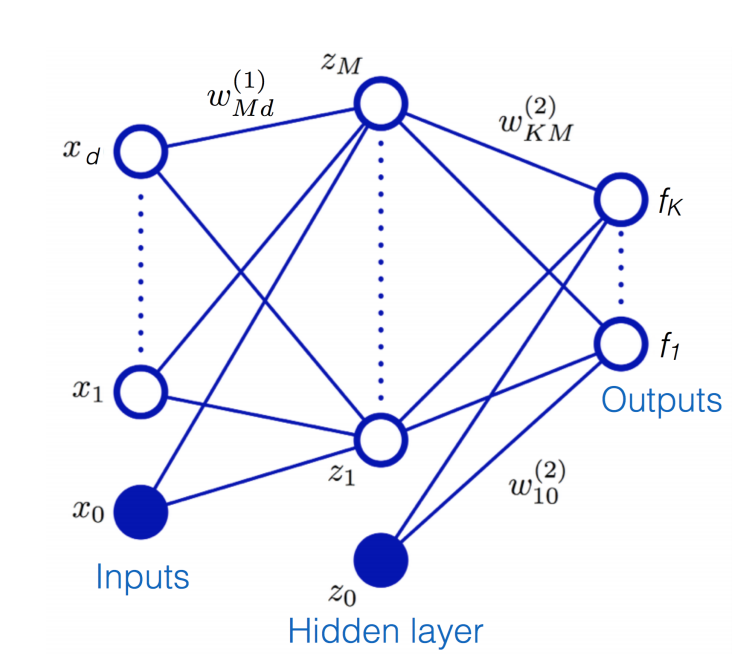
\includegraphics[width=\linewidth]{figures/neural.png}
  \caption{1-hidden layer neural networ taken from Bishop}\label{fig:neural}
\endminipage\hfill
\end{figure}
Figure 1 shows a basic neural network. The $x$ on the left is the input, with each of the $d$ dimensions acting as a separate node. These are then multiplied by the appropriate weights, added to a \textit{bias} (representing $x_0$ here), in order to obtain the \textit{activations} $a_j$ for $1\le j\le M$. These activations are then put through some non-linear map, in this case the sigmoid function, to obtain the values at the first hidden layer $z_j$. Mathematically, this looks like:
$$a_j^{(1)} = \sum_{i=1}^d w_{ji}^{(1)}x_i+w_{j0}^{(1)}$$
$$z_j = g(a_j^{(1)}) = \frac{1}{1 + e^{-a_j^{(1)}}}$$

To arrive at a simple one-hidden-layer neural network, we do this all over again, using our previous hidden layer node values (our $z_j$) instead of our inputs $x_i$ as the inputs to the second layer. The equations for this layer are analogous:
$$a_k^{(2)} = \sum_{j=1}^d w_{kj}^{(2)}x_j+w_{k0}^{(1)}$$
$$f_k = g(a_k^{(2)}) = \frac{1}{1 + e^{-a_k^{(2)}}}$$

In this paper, we will consider a loss function in the form of a negative log likelihood, taking the form:
$$\ell(w) = \sum_{i=1}^N\sum_{k=1}^K\left[-y_k^{(1)}\log(h_k(x^{(i)},w))-(1-y_k^{(1)})\log(1-h_k(x^{(i)},w))\right]$$
If we optimize this directly, however, we will often overfit to the training data (of which we have $n$ samples from $x^{(1)}$ to $x^{(n)}$ - we distinguish these from $x_i$, which are the features of one particular sample that we will consider at a time). Thus, we add a regularization term on the weights $w^{(1)}$ and $w^{(2)}$, so that we try to minimize:
$$J(w) = \ell(w)+\lambda(||w^{(1)}||_F^2+||w^{(2)}||_F^2)$$
\end{document}







